\begin{exercice}[Tracé d'un U dans une feuille]
 \begin{minipage}[c]{0.58\linewidth}
 En cours d'Arts Plastiques, le professeur distribue aux élèves des feuilles carrées de 15 cm de côté. Il leur demande de découper un rectangle de largeur 5 cm pour former la lettre U. 
  \end{minipage} \hfill%
  \begin{minipage}[c]{0.38\linewidth}
  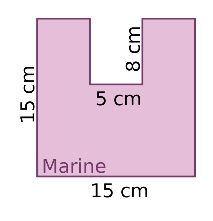
\includegraphics[width=3.1cm]{U_rose}
  \end{minipage} \\
\begin{enumerate}
 \item Marine découpe un rectangle de longueur 8 cm (et de largeur 5 cm). Calcule le périmètre du U de Marine.
 \item Ses amies Alison et Laura ont découpé des rectangles de largeur 5 cm mais de longueurs différentes : celui d'Alison a une longueur de 6,3 cm alors que celui de Laura a une longueur de 9,6 cm. Calcule les périmètres des U d'Alison et de Laura. Quelle partie du calcul est la même pour tous les U ? 
 \item Après tous ces calculs, Kévin remarque que si $L$ désigne la longueur du rectangle en centimètres et $P$ le périmètre du U en centimètres, alors $P = 60 + 2L$ . Calcule $P$ lorsque $L = 7,5 \text{cm}$ et lorsque $L = 10 \text{cm}$.
 \item Priscilla dit : « On peut encore simplifier : $60 + 2 = 62$ donc $P = 62 L$ ». Utilise l'expression proposée par Priscilla pour calculer $P$ lorsque $L = 10 \text{cm}$. Que penses-tu de sa proposition ? Pourquoi ?
 \end{enumerate}
\end{exercice}


\begin{exercice}[Construction d'un escalier]

\vspace{1em}
 \begin{minipage}[c]{0.58\linewidth}
Clémence a fabriqué un escalier de quatre marches à l'aide de briques bleues toutes identiques d'un jeu de construction. Martin a ajouté des briques jaunes (toutes identiques) afin de former le même escalier « à l'envers » au dessus.
  \end{minipage} \hfill%
  \begin{minipage}[c]{0.38\linewidth}
  
\includegraphics[width=3.5cm]{escalier_duplo}
  \end{minipage} \\
\begin{enumerate}
 \item Quel est le nombre de briques bleues utilisées ? Écris-le sous la forme d'une somme.
 \item Clémence rajoute des briques bleues pour obtenir une cinquième marche à son escalier. À son tour, Martin rajoute autant de briques jaunes pour avoir le même escalier « à l'envers ».
 \begin{itemize}
  \item Réalise un dessin représentant les deux escaliers. Ils forment un rectangle.
  \item Quel est alors le nombre total de briques utilisées ? Écris-le sous la forme d'un produit.
  \item Déduis-en la valeur de $1 + 2 + 3 + 4 + 5$.
  \end{itemize}
  \item Sans faire de dessin, donne le nombre total de briques qu'il faudrait si on rajoutait une sixième marche à chacun des deux escaliers. Quel serait alors le nombre de briques bleues ? Déduis-en la valeur de $1 + 2 + 3 + 4 + 5 + 6$.
  \item On appelle $n$ le nombre de marches d'un escalier :
  \begin{itemize}
   \item Écris une expression qui indique le nombre total de briques nécessaires à la construction de deux escaliers de $n$ marches.
   \item Et pour un seul escalier ?
   \item Quelle égalité peut-on alors écrire ?
   \end{itemize}
  \item Combien de briques faut-il pour construire un escalier de 30 marches ? Et pour un escalier de 300 marches ?
 \end{enumerate}
\end{exercice}


\begin{exercice}[La pyramide de Gelo]
\vspace{1em}
 \begin{minipage}[c]{0.58\linewidth}
 Maurice a construit une pyramide de briques Gelo comme ci-dessous. Il y a une brique au premier étage, 4 briques au deuxième étage, 9 briques au troisième étage \ldots
  \end{minipage} \hfill%
  \begin{minipage}[c]{0.38\linewidth}
  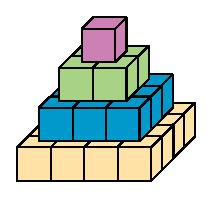
\includegraphics[width=3.2cm]{gelo}
  \end{minipage} \\
\begin{enumerate}
 \item Combien y a-t-il de briques au $4^\text{e}$ étage ? Au $20\text{e}$ étage ? Au $n^\text{e}$ étage ?
 \item Combien y a-t-il de briques au total lorsque la pyramide compte un étage ? Deux étages ? Trois étages ? Quatre étages ? \label{CalcLit_approf}
 \end{enumerate}
Maurice veut savoir combien de briques seront nécessaires pour construire une pyramide à vingt étages. Ne voulant pas faire un gros calcul, il cherche sur internet une formule lui donnant le résultat. Il a trouvé les trois expressions suivantes où $n$ représente le nombre d'étages :
\begin{center} $A = - 6n + 7$ \end{center}
\begin{center} $B = \dfrac{5n^2 - 7n + 4}{2}$ \qquad $C = \dfrac{n(n + 1)(2n +1)}{6}$ \end{center}
Maurice veut alors vérifier la véracité de ces informations.
\begin{enumerate}
\setcounter{enumi}{2}
 \item En testant chacune des formules avec les valeurs trouvées à la question \ref{CalcLit_approf}, quelles sont les formules que l'on peut éliminer d'office ?
 \item Maurice demande à son professeur si la formule non éliminée est exacte. Il lui répond par l'affirmative. Combien de briques sont nécessaires pour construire cette pyramide à vingt étages ?
 \end{enumerate}
\end{exercice}


